\documentclass[english, 11 pt, class=article, crop=false]{standalone}
%\documentclass[english, 11 pt]{report}
\usepackage[T1]{fontenc}
\usepackage[utf8]{luainputenc}
\usepackage{babel}
\usepackage[hidelinks, bookmarks]{hyperref}
\usepackage{geometry}
\geometry{verbose,tmargin=1cm,bmargin=3cm,lmargin=4cm,rmargin=4cm,headheight=3cm,headsep=1cm,footskip=1cm}
\setlength{\parindent}{0bp}
\usepackage{amsmath}
\usepackage{amssymb}
\usepackage{esint}
\usepackage{import}
\usepackage[subpreambles=false]{standalone}
%\makeatletter
\addto\captionsenglish{\renewcommand{\chaptername}{Kapittel}}
\makeatother
\usepackage{tocloft}
\addto\captionsenglish{\renewcommand{\contentsname}{Innhold}}
\usepackage{graphicx}
\usepackage{placeins}
\raggedbottom
\usepackage{calc}
\usepackage{cancel}
\makeatletter
\usepackage{color}
\definecolor{shadecolor}{rgb}{0.105469, 0.613281, 1}
\usepackage{framed}
\usepackage{wrapfig}
\usepackage{bm}
\usepackage{ntheorem}

\usepackage{ragged2e}
\RaggedRight
\raggedbottom
\frenchspacing

\newcounter{lign}[section]
\newenvironment{lign}[1][]{\Large \refstepcounter{lign} \large
	\textbf{\thelign #1} \rmfamily}{\par\medskip}
\numberwithin{lign}{section}
\numberwithin{equation}{section}
\usepackage{xcolor}
\usepackage{icomma}
\usepackage{mathtools}
\usepackage{lmodern} % load a font with all the characters
\usepackage{xr-hyper}
\makeatother
\usepackage[many]{tcolorbox}

%\setlength{\parskip}{\medskipamount}
\newcommand{\parskiplength}{11pt}
%\setlength{\parskip}{0 pt}
\newcommand\eks[2][]{\begin{tcolorbox}[enhanced jigsaw,boxrule=0.3 mm, arc=0mm,breakable,colback=green!30] {\large \textbf{Eksempel #1} \vspace{\parskiplength}\\} #2 \vspace{1pt} \end{tcolorbox}\vspace{1pt}}

\newcommand\fref[2][]{\hyperref[#2]{\textsl{Figur \ref*{#2}#1}}}
\newcommand{\hr}[2]{\hyperref[#2]{\color{blue}\textsl{#1}}}

\newcommand\rgg[2][]{\begin{tcolorbox}[boxrule=0.3 mm, arc=0mm,colback=orange!55] #2 \vspace{1pt} \end{tcolorbox}\vspace{-2pt}}
\newcommand\alg[1]{\begin{align*} #1 \end{align*}}
\newcommand\algv[1]{\vspace{-11 pt} \begin{align*} #1 \end{align*}}
\newcommand\vs{\vspace{-11 pt}}
\newcommand\g[1]{\begin{center} {\tt #1}  \end{center}}
\newcommand\gv[1]{\begin{center} \vspace{-22 pt} {\tt #1} \vspace{-11 pt} \end{center}}
%\addto\captionsenglish{\renewcommand{\contentsname}{Løsningsforslag tentamen R2 H2015}}

% Farger
\colorlet{shadecolor}{blue!30} 

% Figur
\usepackage{float}
\usepackage{subfig}
\captionsetup[subfigure]{labelformat=empty}
\usepackage{esvect}

\newcommand\sv{\textbf{Svar:} \vspace{5 pt} \\}

%Tableofconents
\renewcommand{\cfttoctitlefont}{\Large\bfseries}
\setlength{\cftsubsecindent}{2 cm}
\newcommand\tocskip{6 pt}
\setlength{\cftaftertoctitleskip}{30 pt}
\setlength{\cftbeforesecskip}{\tocskip}
%\setlength{\cftbeforesubsecskip}{\tocskip}

%Footnote:
\usepackage[bottom, hang, flushmargin]{footmisc}
\usepackage{perpage} 
\MakePerPage{footnote}
\addtolength{\footnotesep}{2mm}
\renewcommand{\thefootnote}{\arabic{footnote}}
\renewcommand\footnoterule{\rule{\linewidth}{0.4pt}}

%asin, atan, acos
\DeclareMathOperator{\atan}{atan}
\DeclareMathOperator{\acos}{acos}
\DeclareMathOperator{\asin}{asin}

%Tabell
\addto\captionsenglish{\renewcommand{\tablename}{Figur}}

% Figur
\usepackage[font=footnotesize,labelfont=sl]{caption}
\addto\captionsenglish{\renewcommand{\figurename}{Figur}}

% Figurer
\newcommand\scr[1]{/home/sindre/R/scr/#1}
\newcommand\asym[1]{/home/sindre/R/asymptote/#1}

%Toc for seksjoner
\newcommand\tsec[1]{\phantomsection\addcontentsline{toc}{section}{#1}
	\section*{#1}}
%\newcommand\tssec[1]{\subsection*{#1}\addcontentsline{toc}{subsection}{#1}}
\newcommand\tssec[1]{\subsection*{#1}}
% GeoGebra
\newcommand{\cms}[2]{{\tt #1( #2 )}}
\newcommand{\cm}[2]{{\large \tt #1( #2 )} \gvs \\}
\newcommand{\cmc}[2]{{\large \tt #1( #2 )} \large (CAS)  \gvs \\ \normalsize}
\newcommand{\cmk}[2]{{\large \tt #1( #2 )} \large (Inntastingsfelt)  \gvs \\ \normalsize}

\newcommand\gvs{\vspace{11 pt}}

\newcommand\vsk{\vspace{11 pt}}
\newcommand{\merk}{\vsk \textsl{Merk}: }
\newcommand{\fig}[1]{
\begin{figure}
	\centering
	\includegraphics[scale=0.5]{fig/#1}
\end{figure}
}
\newcommand{\figc}[1]{
		\centering
		\includegraphics[scale=0.5]{fig/#1}
}

% Opg
%\newcommand{\opgt}{\phantomsection \addcontentsline{toc}{section}{Oppgaver} \section*{Oppgaver for kapittel \thechapter}}
\newcounter{opg}
\numberwithin{opg}{section}

\newcommand{\opl}[1]{\vspace{15pt} \refstepcounter{opg} \textbf{\theopg} \vspace{2 pt} \label{#1} \\}



\begin{document}
\subimport{}{rg}
\eqlen
%\setcounter{chapter}{1}
%\tableofcontents
%\chapter{Trigonometri}
\vspace{\parskip}
Mål for opplæringen er at eleven skal kunne
\begin{itemize}
	\item forenkle og løse lineære og kvadratiske likninger i trigonometriske uttrykk ved å bruke sammenhenger mellom de trigonometriske funksjonene
	\item omforme trigonometriske uttrykk av typen $ a \sin kx + b \cos kx $, og bruke dem til å modellere periodiske fenomener
\end{itemize}
\newpage
\section{Vinkler og enhetssirkelen}
\subsection{Vinkel og vinkelmål}\index{vinkel}
Når linjestykker med samme utgangspunkt ikke er parallelle, utspenner de en vinkel $ v $. Vinkelen indikeres ofte ved å tegne en liten sektor mellom linjestykkene:

\subimport{fig/}{grada}

For å måle denne vinkelen er vi tidligere vant med å bruke \textit{grader} ($ ^\circ $)\index{vinkel!målt i grader}. Vi tenker oss da en sirkel som krysser begge linjer, og at omkretsen til denne sirkelen er delt opp i 360 like store buelengder\index{buelengde}, altså $ 360^\circ $. Hvis vi langs sirkelen må gå 60 slike lengder for å komme fra det ene linjestykket til det andre, sier vi at vinkelen er $ 60^\circ $.

\subimport{fig/}{grad}

Ved geometri i praksis er grader gjerne en foretrukket enhet, men i teoretisk matematikk har det \textit{absolutte vinkelmål}\index{absolutt vinkelmål} mange fordeler. Absolutt vinkelmål oppgis i \textit{radianer} (rad)\index{vinkel!målt i radianer}, som vi beregner på følgende måte: \regv

\textsl{Vi sier at vår tenkte sirkel har radius 1 og dermed omkrets $ 2\pi $. Denne sirkelen kalles \textit{enhetssirkelen}\index{enhetssirkelen}. Lengden vi må gå langs (den tenkte) enhetssirkelen for å komme fra det éne linjestykket til det andre, er vinkelmålet i radianer.}

\subimport{fig/}{rad}

Når man skriver vinkler i radianer, er det vanlig å bare oppgi verdien uten benevning\footnote{I noen sammenhenger brukes benevningen \textit{rad}.}, slik som i \fref{radi} $ - $ radianer er jo tross alt bare en \textit{tenkt} lengde og har derfor ingen dimensjon. Og vi tegner selvfølgelig ikke slike sirkler hver gang vi skal framstille en vinkel, men bare  verdien til $ v $ og en liten sektor:

\subimport{fig/}{rad2}

I overgangen mellom grader og radianer er det spesielt fem vinkler det er viktig å huske: 

{	\centering
	\renewcommand{\arraystretch}{2}	
	\begin{tabular}{c|c|c|c|c}
		$ 0^\circ $ & $ 30^\circ $& $45^\circ$ & $ 60^\circ $ & $ 90^\circ$ \\
		\hline
		0&$\dfrac{\pi}{6}$ & $\dfrac{\pi}{4}$ &$\dfrac{\pi}{3}$ & $\dfrac{\pi}{2}$    \\	 
	\end{tabular}
	\captionof{table}{Sammenfallende vinkler målt i grader (øverst) og radianer.}}\regv
\rad
\subsection{Enhetssirkelen som tallinje}
Tenk at noen ber deg tegne hele tallinjen. Dette virker som en umulig oppgave siden tallinjen består av intervallet $ [-\infty, \infty] $. 

\begin{figure}
	\centering
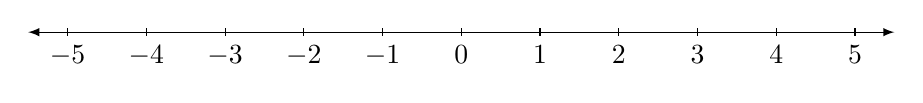
\begin{tikzpicture}[scale=1]
%\tkzInit[xmax=6,ymax=6,xmin=-6,ymin=-6]
\draw[latex -latex] (-5.5,0) -- (5.5,0);
\foreach \x in {-5,...,5}
\draw (\x,0.05) -- (\x ,-0.05) node[anchor=north] {$\x$};
\end{tikzpicture}
\caption{Horisontal tallinje på intervallet $ [-5, 5] $}
\end{figure}

Men hva med dette?\regv

Vi tegner en sirkel med et horisontalt linjestykke trekt mellom sentrum og buen. På enden av dette linjestykket setter vi verdien 0. Videre sier vi at buelengden vi går \textit{mot} klokka har positivt fortegn, mens buelengden vi går \textit{med} klokka har negativt fortegn. 


\fig{enhtl}{}

Vi kan da se på sirkelen som et hjul som har startet på en horisontal tallinje i $ -\infty $ og deretter ''tatt'' alle verdier til seg mens det har rullet mot høyere tall.

\subimport{fig/}{tlin2}

Vi står fritt til å velge en hvilken som helst sirkel til å represenere tallinjen, men et kløktig valg er den nevnte enhetssirkelen\index{enhetssirkelen!som tallinje}. Alle sirkler som heretter blir avbildet vil derfor være sirkler med radius 1. \vsk

Enhetssirkelen som tallinje er selveste grunnlaget for de \textit{trignometriske uttrykkene} vi skal se på i kommende seksjon. Det vil da være noen verdier på interallet $ (-\pi, \pi] $ som blir spesielt viktige, disse er derfor tegnet inn i figuren under:

\fig{unitcirc}{Intervallet  $ (-\pi, \pi] $ avbildet på enhetssirkelen.\label{enh}}

Ekstra verdt å legge merke til i \fref{enh} er symmetrien om horisontallinjen, og at sektoren mellom 0 og et tall på øvre halvdel har en vinkel som, målt i radianer, har samme verdi som tallet.
\section{Trigonometriske uttrykk}
\subsection[Sinus, cosinus og tangens til $ x $]{Sinus, cosinus og tangens til $ \bm x $}\index{sinus}\index{cosinus}
Tiden er inne for å definere  \textit{cosinus} og \textit{sinus} til tallet\footnote{Merk at definisjonen bare er en utvidelse av det du tidligere har lært, hvor du så på sinus og cosinus som forholdstall i rettvinklede trekanter.} $ x $, som vi forkorter til henholdsvis $ \cos x $ og $ \sin x $.\newpage
\sincos \regv
Vi skal straks studere $ \cos x $ og $ \sin x $ nærmere, men bør først gjøre noen forenklinger for kommende figurer. Fordi enhetssirkelen befinner seg i intervallet $ [-1, 1] $ både langs horisontalaksen og vertikalaksen, skal vi kutte akselinjene rett av i disse endepunktene. Og istedenfor å tegne både et punkt og buen som tar oss dit, nøyer vi oss med å skrive $ x $ i enden av buen. Med disse og noen flere små forenklinger blir for eksempel figuren fra definisjonen over seende slik ut:

\subimport{fig/}{forenk}
\newpage
Etterhvert vil vi også bruke begrepet \textit{kjerne}\index{kjerne} om tallet vi finner den trigonometriske verdien av. For eksempel er $ x $ kjernen til cosinusuttrykket $ \cos x $, mens $ kx+c $ er kjernen til sinusutrykket $ \sin (kx+c) $.\vsk

\textbf{Tangens}\bs\index{tangens}
Med $ \cos x $ og $ \sin x $ definert, er det fort gjort å definere \textit{tangens} til et tall $ x $, som vi skriver som $ \tan x $:\regv
\tang
\tssec{Arcuscosinus, arcusinus og arcustangens}\index{arcuscosinus}\index{arcussinus }\index{arcustangens }
Ut ifra figuren knyttet til \eqref{cosdef} og \eqref{sindef} kan vi slutte at $ {\cos \pi = -1}$ (og at $ {\sin \pi =0} $).
\begin{figure}
	\centering
	\subfloat[a)]{\includegraphics[]{\asym{acospi}}}\qquad
	\subfloat[b)]{\includegraphics[]{\asym{acospib}}}	
	\caption{a) $ \pi $ plassert på enhetssirkelen som tallinje. b) I koordinatsystemet samsvarer verdien $ \pi $ med punktet $ (-1, 0) $ }
\end{figure}
Altså er $ \pi $ et tall som har $ -1 $ som cosinusverdi. Dette kan også uttrykkes ved begrepet arcuscosinus, som gjerne forkortes til\footnote{Noen forfattere bruker $ \arccos x$ eller $ \cos^{-1} x$ istedenfor $ \acos x$.} acos. Da skriver vi $ {\acos \pi =-1}$.\vsk

Si videre vi har ligningen
\begin{equation}\label{acosderx}
\acos d=x 
\end{equation}
hvor \y{d\in[-1, 1]}. Å bestemme verdien til $ x $ uten bruk av hjelpemidler er ofte vrient, men vi kan likevel si noe om \textsl{hvor} på enhetssirkelen $ x $ befinner seg:\vsk

Et koordinatsystem plassert i sentrum av enhetssirkelen gir en inndeling i fire sektorer. Disse sektorene kalles første, andre, tredje og fjerde \textit{kvadrant} \index{kvadrant}.\vs

\subimport{fig/}{kvad}

Det er helt avjørende å forstå at vi i trigonometri snakker om tre forskjellige tallinjer, nemlig enhetssirkelen, horisontalaksen og vertikalaksen. Mens \fref{enh} viser tall plassert langs buen til enhetssirkelen, er $ -1 $ og 1 i \fref{kvadr} plassert på horisontal- og vertikalaksen. 1 og $ -1 $ representerer ekstremverdiene til cosinus (horisontalaksen) og sinus (vertikalaksen).\vsk

Av dette observerer vi at hvis \y{d\in[0,1]}, må $ x $ ligge\footnote{Tall med cosinusverdi lik $ -1, 0 $ eller 1 ligger i grensesjiktet mellom to kvadranter.} på buen til første eller fjerde kvadrant. På samme vis må $ x $ ligge på buen til andre eller tredje kvadrant hvis \y{d\in[-1, 0]}. \vsk

Vi innser også at det må finnes flere verdier av $ x $ som kan oppfylle \eqref{acosderx}. For eksempel må det finnes et tall i 4. kvadrant som har samme cosinusverdi som et tall i 1. kvadrant. 
For denne typen ligninger er det likevel vanlig å bare oppgi én løsning, altså en $ x $ liggende enten i første eller andre kvadrant. I denne boka, og på de fleste kalkulatorer, svarer dette til $ {x\in [0, \pi] }$.\vsk

Prinsippet bak arcussinus og arcustangens er akkurat det samme som for arcuscosinus, bare at vi for $ {x=\asin d}$ eller $ {x=\atan d }$ bruker en løsning som ligger i første eller fjerde kvadrant. Vanligst er å oppgi en $ x $ på intervallet $ {\Big[-\frac{\pi}{2}, \frac{\pi}{2}\Big]} $.
\newpage
\arcus
\arcuse
\tssec{Eksaktverdier \label{eksaktverdier}}
Et lite utvalg av sinus-, cosinus- og tangensverdier\footnote{$ \tan x $ er ikke definert for $ {x=\frac{\pi}{2}} $, men $ {\lim\limits_{x\to\frac{\pi}{2} }\tan x =\infty} $} bør vi kjenne til, nemlig følgende:

{\centering		\renewcommand{\arraystretch}{1.5}	
		\begin{tabular}{l|c|c|c|c|c}
			& 0&$\frac{\pi}{6}$ & $\frac{\pi}{4}$ &$\frac{\pi}{3}$ & $\frac{\pi}{2}$    \\
			\hline
			$\sin x$ & 0 &$\frac{1}{2}$ & $\frac{\sqrt{2}}{2}$ & $\frac{\sqrt{3}}{2}$ & 1 \\
			$\cos x$ & 1 & $\frac{\sqrt{3}}{2}$ & $\frac{\sqrt{2}}{2}$ & $\frac{1}{2}$ & 0 \\
			$\tan x$ & 0 &$\frac{1}{\sqrt{3}}$ & $1$ & $\sqrt{3}$ & $ \infty  $
		\end{tabular}
\captionof{table}{Eksaktverdier for sinus, cosinus og tangens av $ x $ \label{eksakt}}}\vsk

Tabellen kan nok virke litt infløkt, men i \hrv{husksincos} finner du et enkelt triks som kan hjelpe deg å huske den.\vsk

Viktig å merke seg er at vi ut ifra denne tabellen også vet om eksaktverdiene for sinus, cosinus og tangens til mange flere tall. Tar vi et blikk tilbake til \fref{enh}, kan vi for eksempel se at $ \frac{\pi}{4} $ og $ \frac{3\pi}{4} $ har samme sinusverdi\footnote{Strengt tatt kan vi ikke være helt sikre på dette ut ifra øyemål, men det blir forklart i \hrs[seksjon]{linlig} at det stemmer.} og at $ {\cos \left(\frac{3\pi}{4}\right)=-\cos \left(\frac{\pi}{4}\right) }$. Slik kan vi ut ifra \hrs[tabell]{eksakt} bestemme de eksakte sinus-, cosinus- og tangensverdiene til alle tallene i \fref{enh}.

\tssec{Trigonometriske identiteter}
Mange trigonometriske uttrykk kan skrives på flere måter, disse omskrivingene kalles gjerne \textit{trigonometriske identiteter}\index{trigonometrisk!identitet}. Et lite utvalg er listet opp under\footnote{For trigonometriske potenser er det vanlig å skrive eksponenten bak selve ''navnet''. For eksempel betyr  $ \sin^2 x $ det samme som $ (\sin x)^2 $. \\ 
\textsl{Obs!} Som nevnt blir $ \sin^{-1}x $ brukt istedenfor $ \asin x $ i noen lærebøker. Da er $ \sin^{-1}x\neq(\sin x)^{-1} $.}:\regv
\trien
\triene
\eks[2]{\label{trigkombeks}Skriv om
\[ 2\sin\left(5x+\frac{2\pi}{3}\right) \]
til et uttrykk bestående av både et cosinus- og et sinus-ledd.\\

\sv
Vi vet at $ {\cos \left(\frac{2\pi}{3}\right)=-\frac{1}{2} }$ og at $ {\sin \left(\frac{2\pi}{3}\right)=-\frac{\sqrt{3}}{2} }$, derfor kan vi skrive:
\alg{
	2\sin\left(5x+\frac{2\pi}{3}\right) &= 
	2\left(\sin (5x) \cos \left(\frac{2\pi}{3}\right)+\cos(5x)\sin\left(\frac{2\pi}{3}\right)\right) \\
	&= 2\left(\sin (5x)\cdot\left(-\frac{1}{2}\right)+\cos(5x)\frac{\sqrt{3}}{2}\right)\\
	&= \sqrt{3}\cos(5x)-\sin(5x) 
	}\vds
	}
\newpage
\tssec{Sinus og cosinus kombinert \label{trigkomb}}%på side \pageref{trigkombeks} 
Av \textsl{Eksempel 2} på forrige side merker vi oss at når et sinus-uttrykk kan skrives om til et kombinert sinus- og cosinusuttrykk, må det også gå an å gå andre veien:\regv
\komb
\kombe

\section{Lineære ligninger \label{linlig}}
I forrige seksjon så vi på sinus-, cosinus- og tangensverdiene til tall på intervallet $ [-\pi, \pi) $. Vi skal nå gå over til å løse trigonometriske ligninger. Da er det viktig å ta hensyn til at løsningene liksågodt kan ligge utenfor dette intervallet, og at mange forskjellige tall kan oppfylle samme ligning. \vsk

De første ligningene vi skal se på kalles \textit{lineære} trigonometriske ligninger. \index{trigonometrisk!ligning!lineær} Navnet kommer av at de trigonometriske uttrykkene som $ \sin x $, $ \cos x $ osv. bare forekommer i første potens\footnote{Tallet $ a^1 $ er $ a $ i første potens, mens $ a^2 $ er $ a $ i andre potens osv.}.
\tssec{Cosinus-ligninger}
La\footnote{Når $ {d\in\{-1, 1\}} $ får vi to spesialtilfeller av ligningen, men resonnementet for å finne løsningene er helt analogt til det som gis ved $ {d\in(-1, 1)} $.} $ {d\in(-1, 1)} $. Vi ønsker å finne alle løsninger av ligningen
\[ \cos x=d \label{cosslig} \]
Hvis $ {0\leq d <1}$, må vi ha en løsning $ {x=v_1} $ i første kvadrant (se \fref{kvadr} og \textsl{\ref{cosligfig}}). Men om vi fra 0 går en buelengde $ v_1 $ i negativ retning, har vi kommet like langt langs horisontalaksen, derfor må også $ {x=-v_1} $ være en løsning.\vsk

Hvis vi derimot har at $ {-1< d<0} $, må vi ha en løsning $ {x=v_2} $ i andre kvadrant, og da må også ${ x=-v_2} $ være en løsning.
\subimport{fig/}{coslig}
Og hva nå om vi står i punktet til den ene av løsningene og derifra vandrer $ 2\pi $ buelengder i enten negativ eller positiv retning? Jo, da er vi tilbake til det eksakt samme punktet. Har vi én løsning kan vi altså finne en ny løsning ved å legge til et heltalls antall $ 2\pi $. Alle heltallene, nemlig følgen $ \{...,-2, -1, 0, 1, 2, ... \} $, skriver vi som $ \mathbb{Z} $.\vsk

Til slutt tar vi med oss at siden cosinusverdier handler om horisontalkoordinaten til et punkt på enhetssirkelen, vil vi ikke få \textit{reelle}\footnote{Vi kommer tilbake til dette begrepet i \hrs[kapittel]{Differensialligninger}, se s. \pageref{rkmpstart}.} svar hvis $ {d\not \in [1,1]} $.\regv

\coslig
\coslige
\cosligeto
\tssec{Sinusligninger}
Gitt ligningen 
\begin{equation}
\sin x = d \label{slig}
\end{equation}
Hvis $ {0\leq d <1}$, må vi ha en løsning $ {x=v_1} $ i første kvadrant (se \fref{sinligfig}). Men om vi starter i $ \pi $ og går en buelengde $ x_1 $ i negativ retning, har vi kommet akkurat like høyt langs vertikalaksen, og dermed må også ${x=\pi-v_1} $ være en løsning.\vsk

Er derimot $ {-1< d <0}$, må en løsning $ x=v_2 $ ligge i fjerde kvadrant. Da er også $ x=\pi-v_2 $ en løsning.
\subimport{fig/}{sinlig}
Og vandrer vi $ \pm 2\pi $ finner vi stadig nye løsninger.\regv
\sinlig
\sinlige
\tssec{Tangensligninger}
Gitt ligningen
\[ \tan x = d \]
I én av kvadrantene må det finnes en løsning ${ x=v }$. Hvis vi vandrer en buelengde $ \pi $ fra denne løsningen, kommer vi til et tall som har sinusverdi $ {-\sin v} $ og cosinusverdi $ {-\cos v} $.
\subimport{fig/}{tanlig}
Dette tallet har altså samme tangensverdi som $ v $, og må derfor også være en løsning. Og vandrer vi $ \pm \pi $ herfra får vi stadig nye løsninger.\newpage
\tanlig
\tanlige
\subsection[$ a\sin (kx) + b\cos (kx) =0 $]{\boldmath $ a\sin (kx) + b\cos (kx) =0 $}
Vi har hittil sett på ligninger med ett sinus-, cosinus- eller tangensuttrykk, men ofte kommer vi ut for ligninger som har kombinasjoner av disse. La oss prøve å løse ligningen
\begin{equation}\label{trikomblig0}
a\sin (kx) + b\cos (kx) =0  
\end{equation}
hvor $ a $, $ b $ og $ k $ er konstanter forskjellige fra 0. \vsk

Det første vi observerer er at hvis $ \cos(kx)=0 $, er\footnote{Se \eqref{coslig}.} $ x=\frac{1}{k}\left(\pm\frac{\pi }{2}+2\pi n\right) $. I så tilfelle er $ \sin
(kx)=\pm 1 $, og da får vi at
\alg{
a\sin (kx) + b\cos (kx) =\pm a+0 \neq 0
	}
Dette funnet gjør at vi trygt kan dele (\ref{trikomblig0}) med $ \cos (kx) $:
\alg{
 \frac{a\sin (kx) + b\cos (kx)}{\cos (kx)} &=\frac{0}{\cos (kx)}	\br
 \frac{a\sin (kx)}{\cos kx} + b &= 0 \br
 a\tan (kx) &= -b \br
 \tan (kx) &= -\frac{b}{a}
	}
Vi har nå endt opp med en tangensligning med løsninger gitt ved \eqref{tansols}.
\asinbcos
\eks{
Løs ligningen
\[ \sqrt{3}\sin (\pi x) + \cos (\pi x) = 0 \] \vs
\sv
Vi starter med å dele på $ \cos(kx) $:
\alg{
\frac{\sqrt{3}\sin (\pi x) + \cos (\pi x)}{\cos (\pi x)} &= \frac{0}{\cos(\pi x)} \br
\sqrt{3}\tan (\pi x) + 1 &= 0 \br
\tan (\pi x) &= -\frac{1}{\sqrt{3}}
	}
Siden $ \atan\left(-\frac{1}{\sqrt{3}}\right)=-\frac{\pi}{6} $, er
\alg{
\pi x &= -\frac{\pi}{6}+\pi n	\br
x &= n - \frac{1}{6}
}\vsb
	}
\subsection[$ a\sin (kx) + b\cos (kx) =d $]{\boldmath $ a\sin (kx) + b\cos (kx) =d $}
En noe mer avansert utgave av \eqref{asinbcos00} får vi hvis høyresiden er en konstant $ d $ istedenfor 0. Da utnytter vi \eqref{rsin} for å omskrive ligningen til en form vi kan løse:\regv
\asinbcosd
\eks{
	Løs ligningen
	\[ \sin (3x) + \cos (3x) = \sqrt 2 \]\vs
	\sv
	Vi starter med å finne det kombinerte sinusuttrykket for venstresiden av ligningen:\\
\parbox[t][][t]{0.32\linewidth}{\alg{
		r &= \sqrt{1^2 + 1^2}	\\
		&= \frac{\sqrt{2}}{2}\br
		&= \sqrt{2}
}}
\parbox[t][][t]{0.32\linewidth}{
	\alg{		
		\cos c &= \frac{1}{\sqrt{2}}\br
		&= \frac{1}{\sqrt{2}}\frac{\sqrt{2}}{\sqrt{2}}\br
		&= \frac{\sqrt{2}}{2}	
}
}
\parbox[t][][t]{0.32\linewidth}{\alg{\sin c &= \frac{1}{\sqrt{2}}}}	
	$c= \frac{\pi}{4} $ oppfyller kravene over, dermed er
	\alg{
		\sqrt{2}\sin\left(3x+\frac{\pi}{4}\right)&=\sqrt{2} \br
		\sin\left(3x+\frac{\pi}{4}\right)&=1
	}
	Altså har vi at
	\alg{
		3x + \frac{\pi}{4} &= \frac{\pi}{2} + 2\pi n\br
		x &= \frac{\pi}{3}\left(\frac{1}{4}+2n\right)
	}\vs
}
\section{Kvadratiske ligninger}
Vi skal nå se på to typer ligninger der sinus-, cosinus- eller tangensuttrykk opptrer i andre potens. Uttrykk i andre potens kalles \textit{kvadrerte}\index{kvadrert} uttrykk, derav navnet \textit{kvadratiske ligninger}\index{trigonometrisk!ligning!kvadratisk}.

\tssec{Løsning ved abc-formelen}
La oss forsøke å løse ligningen
\begin{equation}
2\sin^2 x -3\sin x-2 \label{sin2}=0
\end{equation}
Vi observerer at (\ref{sin2}) er en andregradsligning for $ \sin x $ (erstatt $ \sin x $ med $ u $ hvis du syns det er vanskelig å se). Vi kan derfor bruke \textit{abc}-formelen til å løse ligningen med hensyn på $ \sin x $, og finner da at:
\[ \sin x = \frac{1}{2} \quad\vee\quad \sin x = -2 \]
Altså har vi to sinusligninger vi nå må finne løsningene til. Vi vet at $ \asin \frac{1}{2} = \frac{\pi}{6} $, dermed er (se (\ref{sinlig})):
\[ x = \frac{\pi}{6}+2\pi n \quad \vee \quad x = \pi-\frac{\pi}{6}+\frac{2\pi}{n}=\frac{5\pi}{6}+\frac{2\pi}{n}\]
Derimot er det ingen \textit{reelle} tall som kan oppfylle ligningen \\ $ {\sin x=-2} $, vi anser derfor (\ref{sin2}) som ferdig løst.\regv
\kvaden
\newpage
\kvadene
\eks[2]{
Løs ligningen
\[ 4\cos^2 (\pi x) -\sqrt{48}\cos (\pi x) +  3=0 \]\vs
\sv 
Av $ abc $-formelen er
\alg{
	\cos x &= \frac{-(-\sqrt{48})+\sqrt{\sqrt{48}^2-4\cdot4\cdot3}}{2\cdot4} \br
	&= \frac{\sqrt{48}}{8} \br
	&= \frac{\sqrt{16}\sqrt{3}}{2\cdot 4} \br
	&= \frac{\sqrt{3}}{2}
}
Fordi $ \acos\left(\frac{\sqrt{3}}{2}\right)=\frac{\pi}{6} $,  har vi at
\alg{
\pi x &= \pm \frac{\pi}{6}+2\pi n \\
&= \pm \frac{1}{6}+2 n
}\vsb
}
	
\tssec{Kvadrater av sinus og cosinus kombinert}
Vi går videre til å studere ligningen
\begin{equation}
3 \cos^2 (2x) + 5\sin^2 (2x) = 4 \label{kvadd2}
\end{equation}
Fra (\ref{1}) vet vi at $ 1 = \cos^2 (2x)+\sin^2 (2x) $, derfor kan vi skrive:
\alg{
	4 &= 4\cdot1 \\
	&= 4\left(\cos^2 (2x)+\sin^2 (2x)\right)
}
Kanskje litt overraskende forenkler dette ligningen vi ønsker å løse:
\alg{
	3 \cos^2 (2x) + 5\sin^2 (2x) &= 4\left(\cos^2 (2x)+\sin^2 (2x)\right) \\
	-\cos^2 (2x) + \sin^2 (2x) &= 0}
Videre deler\footnote{Vi observerer at \eqref{kvadd2} ikke har en løsning (sjekk selv!) når $ {\cos (2x)=0} $. Derfor er vi sikre på å unngå nulldivisjon.} vi ligningen med $ \cos^2 (2x) $:
\alg{
	\frac{-\cos^2 (2x) + \sin^2 (2x)}{\cos^2 (2x)}&= \frac{0}{\cos^2(2x)} \\
	-1 + \tan^2 (2x) &= 0 \\
	\tan^2 (2x) &= 1 \\
	\tan(2x)&= \pm 1
}
Siden $ {\atan 1 = \frac{\pi}{4}} $ og $ {\atan (-1) = -\frac{\pi}{4}} $, har vi at
\alg{
	2x &= \pm\frac{\pi}{4} + \pi n \br
	x &= \frac{1}{2}\left(\pm\frac{\pi}{4} + \pi n\right)
}

\kvad
\eks{
Løs ligningen
\[ -3\cos^2(5 x)+\sin^2(5 x)=-2 \] \vs
\sv \vs
\algv{
-3\cos^2(5 x)+\sin^2(5 x)&=-2(\cos^2 (5 x) + \sin^2 (5 x)) \\
-\cos^2(5 x)+3\sin^2(5 x)&= 0 \\
- 1 + 3 \tan^2 (5 x) &= 0 \\
\tan^2(5 x) &=\frac{1}{3} \br
\tan(5 x) &=\pm \frac{1}{\sqrt{3}}
}
Siden $ \atan\left(\frac{1}{\sqrt{3}}\right)=\frac{\pi}{6} $ og $ {\atan\left(-\frac{1}{\sqrt{3}}\right)}=\frac{\pi}{6} $, har vi at
\alg{
5 x &= \pm \frac{\pi}{6}+\pi n\br
x &= \pm \frac{1}{5}\left(\frac{\pi}{6}+\pi n\right)
}\vsb
}

\section{Trigonometriske funksjoner \label{trifunksjoner}}
\tssec{Cosinusfunksjoner}\index{cosinus!-funksjon}
La oss studere funksjonen
\nreq{
	f(x) = a\cos (kx+c) + d 	
}
hvor $ a $, $ k $, $ c $ og $ d $ er konstanter. Dette kaller vi en \textit{cosinusfunksjon}. I \fref{fcosfig} vises grafen til
\[ f(x)= 2\cos\left(\frac{\pi}{2}x-\pi \right)+1  \]
\subimport{fig/}{fcos} 
Av figuren merker vi oss følgende:
\begin{itemize}
	\item horisontalavstanden fra et toppunkt\footnote{Det er antatt at begrep som toppunkt, ekstremalpunkt o.l. er kjent for leseren. Hvis ikke finnes definisjonen av disse i \hrv{pktpgrf}} til et annet er 4. Denne avstanden kalles \textit{perioden}\index{periode} (eventuelt \textit{bølgelengden}\index{bølgelengde}).	
	\item topp- og bunnpunktene har den samme vertikalavstanden til linja $ {y=1} $, som kalles  \textit{likevektslinja}\index{likevektslinje} til grafen. Verdien til likevektslinja samsvarer med konstantleddet\index{konstantledd} til $ f $.
	\item vertikalavstanden fra likevektslinja til et toppunkt er $ 2 $, denne avstanden kalles \textit{amplituden}\index{amplitude}. Verdien til amplituden samsvarer med faktoren foran cosinusuttrykket.
\end{itemize}
Om vi ikke visste uttrykket til $ f $, kunne vi altså ut ifra  \fref{fcosfig} og punktene over sett at\footnote{Som vi straks skal se, kunne $ a $ også vært $ -2 $. Men når vi skal finne et cosinusuttrykk, kan vi alltid finne et uttrykk med ${ a>0} $ som vil samsvare med grafen.} $ {a=2} $ og $ {d=1} $. Men hva med $ k $ og $ c $? \vsk

La oss starte med det enkleste: Når vi kjenner perioden $ {P=4 }$, kan vi finne \textit{bølgetallet}\index{bølgetall} $ k $ ut ifra følgende relasjon:
\alg{
	k &= \frac{2\pi}{P} \br
	&= \frac{2\pi}{4} \br
	&= \frac{\pi}{2}	
}
For å bestemme $ c $ gjør vi denne observasjonen: En cosinusfunksjon med positiv $ a $ må ha et toppunkt der hvor $ {kx+c=0} $ (fordi $ \cos 0=1 $). Da $ f $ har et toppunkt der $ {x=2} $, må vi ha at
\alg{
	\frac{\pi}{2}\cdot 2 +c &= 0 \\
	c &= -\pi
}
En endring i $ c $ vil forskyve cosinusfunksjonen horisontalt, $ c $ kalles derfor \textit{faseforskyvningen}\index{faseforskyvning} (eventuelt bare \textit{fasen}\index{fase}).\vsk

La oss også kort studere grafen til
\[ {g(x) = -2\cos\left(\frac{\pi}{2}x-\pi\right)+1} \]
\subimport{fig/}{gcos}

Den eneste forskjellen på uttrykkene til $ f $ og $ g $ er at $ g $ har faktoren $ -2 $ foran cosinusuttrykket. Vertikalavstanden fra likevektslinja til et toppunkt er likevel 2 også for $ g $, som derfor har 2 som amplitude. For en hvilken som helst cosinusfunksjon er altså $ |a| $ lik verdien til amplituden. Fordi $ a $ er negativ, har $ g $ et toppunkt når $ {kx+c=\pi} $ (siden $ \cos \pi=-1 $).\newpage
\rg[Cosinusfunksjonen]{
	En funksjon $ f(x) $ på formen
	\begin{equation}\label{cosinusfunksjonen}
	f(x)= a \cos (kx+c) + d 
	\end{equation}
	kalles en cosinusfunksjon med amplitude $ |a| $, bølgetall $ k $, fase $ c $ og likevektslinje $ y=d $.
	\subimport{fig/}{fcos2}
	Hvis $ f $ har to naboliggende toppunkt $ x_1 $ og $ x_2 $, er
	\begin{equation}\label{perioden}
	P=x_2-x_1
	\end{equation}
	og
	\begin{equation}\label{ker2pioverP}
	k = \frac{2\pi}{P} 
	\end{equation}
	Videre kan $ c $ finnes ut ifra ligningen
	\begin{equation}\label{c}
	k x_1+ c = 0 
	\end{equation}
	Funksjonen har ekstremalpunkter for alle $ x $ der
	\begin{equation}\label{cosmax}
	kx +c = 2\pi n \quad \vee\quad kx+c = \pi + 2\pi n
	\end{equation}
	for alle $ n\in \mathbb{Z} $.
}
\newpage
\eks[1]{
Grafen til cosinusfunksjonen $ f $ er skissert i figuren under.
\subimport{fig/}{cosopg}
Finn et uttrykk for $ f $. \\

\sv
Vi observerer at verdiene til $ f $ varierer mellom 1 og 5. Dette betyr at likevektslinja er $ {y=\frac{1+5}{2}=3} $ og at amplituden er $ {\frac{5-1}{2}=2} $. Vi legger også merke til at horisontalavstanden mellom to toppunkt er $ {2\pi-(-2\pi)=4\pi} $, som altså er bølgelengden. Dermed er\vspace{-5pt}
\[f(x)= a\cos(kx+c)+d \]
hvor $ {a=2} $, $ {d=3} $ og $ {k=\frac{2\pi}{4\pi}=\frac{1}{2}} $. Fasen $ c $ finner vi ved å observere at $ f $ har et toppunkt for $ {x=2\pi }$. Cosinusverdien til $ f $ må være 1 i dette punktet, og da er
\alg{
	kx+c&=0\\
\frac{1}{2}\cdot2\pi +c&= 0 \\
c&=-\pi 
}
Uttrykket til $ f $ blir da\vspace{-5pt}
\[f(x)= 2\cos\left(\frac{1}{2}x-\pi\right)+3 \] \vs
}
\newpage
\eks[2]{
	En tilnærming for høy- og lavvann i Molde er gitt ved \\funksjonen 
	\[ f(x)=128+80\cos\left(\frac{3\pi}{37}x\right) \]
	hvor $ f $ angir cm over sjøkartnull\footnote{Sjøkartnull er som regel satt til den laveste vannstanden som kan oppnås ut ifra astronomiske betingelser (flo og fjære er i stor grad betinget av hvordan jorda, sola og månen står i forhold til hverandre).} $ t $ timer etter et gitt referanse-tidspunkt. Referansetidspunktet er valgt slik at det ved $ {t=0} $ var høyvann (flo). \os
	\textbf{a)} Hva er vannstanden i Molde når det er lavvann (fjøre)?\os
	\textbf{b)} Hvor lang tid er det mellom flo og fjøre? 
	
	\sv
	\textbf{a)} En cosinusfunksjon har lavest verdi når cosinusuttrykket har verdien $ -1 $. Den laveste verdien til $ f $ er derfor $ {128-80=48} $. Når det er fjære er altså vannstanden 48\,cm over sjåkartnull.\vsk
	
	\textbf{b)} Av \eqref{ker2pioverP} har vi at perioden $ P $ er gitt som
	\[ P=\frac{2\pi}{k} \]
	I dette tilfellet er $ k=\frac{3\pi}{37} $, altså er
	\alg{
	P&=\frac{37}{3}\\
	&=12+\frac{1}{3}
}
Følgelig er det 12 timer og 20 minutter mellom to etterfølgende tipspunkt for flo. Dette betyr at det er 6 timer og 10 minutter mellom flo og fjære.	
}
\newpage
\tssec{Sinusfunksjoner}\index{sinus!-funksjon}
Funksjoner på formen
\[ f(x) = a\sin (kx+c)+d\]
kalles \textit{sinusfunksjoner}. Amplituden, bølgetallet og likevektslinjen finner vi på akkurat samme måte som for cosinusfunksjoner.\vsk

Fasen finner vi derimot ved å observere at en sinusfunksjon må ha en maksimalverdi der \begin{itemize}
	\item  $ {kx+c=\frac{\pi}{2}} $ hvis $ a $ er positiv \big(fordi $ {\sin \frac{\pi}{2}=1} $\big).
	\item $ {{kx+c = -\frac{\pi}{2}} }$ hvis $ a $ er negativ \big(fordi $ \sin \left(-\frac{\pi}{2}\right)=-1 $\big).
\end{itemize}
\sinf
\newpage
\eks{
	Gitt funksjonen 
	\[  f(x)= 2 \cos (3x+\pi)+1 \]
	\textbf{a)} Skriv om $ f $ til en sinusfunksjon. \os
	\textbf{b)} Finn $ x$-verdiene til toppunktene til $ f $.\\
	
	\sv
	\textbf{a)} Det eneste vi må sørge for er å gjøre om cosinusuttrykket til et sinusuttrykk. Av (\ref{cossomsi}) vet vi at
	\alg{
		\cos(3x+\pi)&= \cos\left(3x+\pi+\frac{\pi}{2}-\frac{\pi}{2}\right)\\
		&= \sin\left(3x+\pi+\frac{\pi}{2}\right)	\\
		&= \sin\left(3x+\frac{3\pi}{2}\right)
	}
	Dermed er
	\[ f(x) = 2\sin\left(3x+\frac{3\pi}{2}\right)+1\]
	\textbf{b)} Fordi sinusuttrykket multipliseres med det positive tallet 2, må toppunktene være der hvor sinusuttrykket blir 1. Da er $ x $ gitt ved ligningen
	\alg{
		kx + c &= \frac{\pi}{2}+2\pi n
	}	
	Vi får derfor at
	\alg{
		3x + \frac{3\pi}{2} &= \frac{\pi}{2}+2\pi n \br
		3x &= 2\pi n -\pi \br
		x &= \frac{\pi}{3}(2n-1)
	}\vs
}

\tssec{Tangensfunksjoner}\index{tangens!-funksjon}
Vi avslutter seksjonen om trigonometrisk funksjoner med \textit{tangensfunksjoner}, nemlig funksjoner $ f $ på formen
\[ f(x)= a\tan(kx+c)+d \]
Når $ x $ går mot $ \frac{\pi}{2}$, går $ \sin x $ mot 1 og $ \cos x $ mot 0. Siden $ {\tan x = \frac{\sin x}{\cos x}} $, vil $ f $ da vil gå mot uendelig. Derfor er det ikke mulig å angi noen amplitude for tangensfunksjonen. Dette betyr også at funksjonen vil oppføre seg asymptotisk.\vs
\fig{tanf}{Grafen til $ {f(x)=\tan(\pi x) }$ på intervallet $ {x\in [-2, 2]} $.\label{ftan}}
Det spesielle med tangensfunksjoner er at den asymptotiske oppførselen gjentar seg med den samme avstanden, altså en periode $ P $ (i \fref{ftan} er $ {P=1} $). Til forskjell fra  sinus- og cosinusfunskjoner er perioden her gitt av formelen
\[ P=\frac{\pi}{k} \]
Med en litt annen tolkning enn tidligere kan man også se på ${ y=d} $ som en likevektslinje, men for tangensfunksjoner er det asymptotetene og perioden som er av størst interesse. \regv
\tanf

\newpage
\tsec{Forklaringer}
\subsection*{Trigonometriske identiteter}
{\boldmath $ \cos(-x)=\cos x$ \textbf{og} $ \sin(-x)=-\sin x $} \bs
Disse to identitetene følger direkte av definisjonen av sinus og cosinus og symmetrien om horisontal- og vertikalaksen.\vsk

{\boldmath $ \cos^2 x + \sin^2 x = 1 $}\bs
I enhetssirkelen er $ \pm \cos x $ og $\pm  \sin x $ katetene i en rettvinklet trekant der hypotenusen har lengde 1. Identiteten følger altså direkte av Pytagoras’ setning. \vsk

{\boldmath$  \cos(u-v)= \cos u\cos v + \sin u\sin v $} \bs

Denne forklaringen bygger på vektorer i planet, som det er antatt at leseren kjenner fra tidligere matematikkurs.\vsk

Gitt to vektorer $ \vec{b} $ og $ \vec{r} $, begge med lengde 1. Disse tegner vi inn i enhetssirkelen med utspring i sentrum. Den horisontale diameteren danner vinkelen $ u$ med $ \vec{b} $ og vinkelen $ v $ med $ \vec{r} $. 
\fig{cosuv}{Vektorene $ \vec{b}$ (blå) og $ \vec{r} $ (rød). \label{cosuvfig}}
Husk nå at en vinkel oppgitt i radianer representerer en buelengde langs enhetssirkelen (selv om vi i \fref{cosuvfig} har indikert vinklene innenfor omkretsen for å unngå overlapping). Av definisjonen til sinus og cosinus (se ligning (\ref{sindef}) og (\ref{cosdef}))) har vi at
\alg{
	\vec{b}=[\cos u, \sin u]	\\
	\vec{r}= [\cos v, \sin v]
	} 
Vinkelen $ \angle(\vec{b}, \vec{r}) $ utspent av to vektorer i planet er gitt som
\[ \cos \angle(\vec b, \vec r) = \frac{\vec{b}\cdot \vec{r}}{|\vec{b}||\vec{r}|} \]
Hvis\footnote{Vinkelen mellom vektorer er bare definert på intervallet $ [0, \pi] $.} $ (u-v)\in[0, \pi] $, er $ \angle(\vec b, \vec r)=u-v $, og dermed er
\alg{
	\cos \angle(\vec b, \vec r) &= \cos (u-v)\br
	&=\frac{[\cos u, \sin u] \cdot [\cos v, \sin v] }{1\cdot1} \br
	&= \cos u\cos v + \sin u\sin v
	}
Det er fristende å si at vi er i mål, men vi har ikke
sjekket hva som skjer hvis $ {\pi<u-v\leq2\pi} $. Det er
heldigvis ingen radikal endring, for-skjellen blir bare at 
$ {u-v=2\pi- \angle(\vec b, \vec r)}$. Og siden ${\cos
(2\pi-x)=\cos x} $ (forklar for deg selv hvorfor), har vi at
\alg{
	\cos(u-v)&=\cos\left(2\pi- \angle(\vec a, \vec b)\right) \\
	&= \cos \angle(\vec b, \vec r) \\
	&= \cos u\cos v + \sin u\sin v
}
Nå har vi altså vist at (\ref{cuv}) gjelder for alle $ u-v\in[0, 2\pi] $. Hvis $ u-v $ ligger utenfor dette intervallet, må det finnes et tall $ 2\pi n $, hvor $ n\in \mathbb{Z} $, som er slik at $ (u-v+2\pi n) \in [0, 2\pi]$. Da kan vi skrive
\alg{
\cos(u-v)&=\cos(u-v+2\pi n) \\
&= 	\cos u\cos (v+2\pi n) + \sin u\sin (v+2\pi n) \\
&= \cos u\cos v + \sin u\sin v
	}
Dermed er (\ref{cuv}) vist for alle $ (u-v) \in \mathbb{R}$. \vsk

\bm{$\cos (u+v)=\cos u \cos v - \sin u \sin v$}
\begin{align*}
\cos (u-v)&= \cos (u-(-v)) \\
&= \cos u \cos (-v) + \sin u \sin (-v) \\
&= \cos u \cos v - \sin u \sin v 
\end{align*} \\

{\boldmath $ \cos\left(u-\frac{\pi}{2}\right)=\sin u $}
\alg{
	\cos\left(u-\frac{\pi}{2}\right)
	&=\cos u \cos\left(\frac{\pi}{2}\right)+\sin u \sin\left(\frac{\pi}{2}\right)\\
	&= \sin u
	}

{\boldmath $ \sin \left(u + \frac{\pi}{2}\right)=\cos u $} 
\alg{
	\sin \left(u+\frac{\pi}{2}\right) &= \cos\left(u+\frac{\pi}{2}-\frac{\pi}{2}\right)	\\
	&= \cos u
	}
\bm{$\sin (u+v)=\cos u\sin v + \sin u \cos v$}\bs
Vi tar først med oss at (det får bli opp til leseren selv å bekrefte dette):
\[ \cos \left(u+\frac{\pi}{2}\right)=-\sin u \]
Da kan vi videre skrive
\begin{align*}\
\cos \left(u+ v+\frac{\pi}{2}\right) &= \cos u \cos \left(v+\frac{\pi}{2}\right) - \sin u \sin\left(v+\frac{\pi}{2}\right) \\
&= -(\cos u \sin v + \sin u \cos v )
\end{align*} 
\\
Siden  $ \cos \left(u+ \left(v+\frac{\pi}{2}\right)\right) = -\sin (u+v) $, har vi nå at
\[\sin (u+v) = \sin u \cos v +\cos u \sin v \]

\bm{$\sin (u-v)=\sin u \cos v-\cos u \sin v$} \label{sin2xbevis}
\begin{align*}
\sin(u-v) =&=\sin (u+(-v)) \\
&= \sin u \cos (-v) + \cos u \sin (-v) \\
&= \sin u \cos v - \cos u \sin v 
\end{align*}

{\boldmath $ \sin (2u)=2\sin u \cos u $}
\alg{
	\sin(2x) &= \sin(x+x) \\&= \sin x\cos x+\sin x + \cos x \\
	&= 2\sin x \cos x
}

{\boldmath $ \cos\left(x-\frac{\pi}{2}\right)=\sin x $}
\alg{
	\cos\left(x-\frac{\pi}{2}\right) &= \cos x\cos\left(\frac{\pi}{2}\right)+\sin x \sin\left(\frac{\pi}{2}\right) \\
	&= \sin x
}

{\boldmath $ \sin\left(x+\frac{\pi}{2}\right)=\cos x $}
\alg{
	\sin\left(x+\frac{\pi}{2}\right) &= \sin x\cos\left(\frac{\pi}{2}\right)+\cos x \sin\left(\frac{\pi}{2}\right) \\
	&= \cos x
}

\subsection*{Sinus og cosinus kombinert}
Gitt uttrykket
\begin{equation}
a \cos (kx) + b \sin (kx) \label{sc}
\end{equation}
Vi vet at (se (\ref{suv}))
\begin{equation}
r \sin(kx+c)= r\sin c\cos (kx) + r\cos c \sin (kx)  \label{s}
\end{equation}
Uttrykkene fra ligning (\ref{sc}) og (\ref{s}) er like hvis
\begin{align}
a &= r\sin c \label{a} \\
b &= r\cos c \label{b}
\end{align}
Kvadrerer vi ligning (\ref{a}) og (\ref{b}), får vi at
\begin{align}
a^2 &= r^2\sin^2 c \label{ab1}\\
b^2 &= r^2\cos^2 c \label{ab2}
\end{align}
Hvis vi nå legger sammen ligning (\ref{ab1}) og (\ref{ab2}), finner vi et uttrykk for $r$:
\alg{
	r^2\sin^2 c+r^2\cos^2 c &= a^2 +b^2 \\
	r^2(\sin^2 c+\cos^2 c) &= a^2 +b^2 \\
	r^2 &= a^2+b^2 \\
	r &= \pm \sqrt{a^2+b^2} 	
}
Hvis vi velger den positive løsningen for $ r $, får vi at
\alg{r &=\sqrt{a^2+b^2} \br
	\cos c &= \frac{b}{r} \br
	\sin c &= \frac{a}{r}}
\newpage
\subsection*{Trigonometriske funksjoner}
\textbf{Tallet} {\boldmath $ k $} \bs
Vi skal nå vise hvorfor vi for en cosinusfunksjon har relasjonen $ {k=\frac{2\pi}{P}} $. Det samme resonnementet kan brukes for en sinusfunksjon, og et veldig lignende et kan brukes for å vise at $ {k=\frac{\pi}{P}} $ for en tangensfunksjon.\vsk

La oss tenke oss en cosinusfunksjon med $ kx+c $ som kjerne. Si videre at $ x_1 $ og $ x_2 $ er $ x $-verdien til to naboliggende toppunkt. 
\subimport{fig/}{fcos3} 
Siden et nytt toppunkt kommer for hver gang vi legger til $ 2\pi $ i kjernen, vet vi at
\algv{
	kx_1+c + 2\pi &=kx_2+c \\
	k(x_2-x_1) &= 2\pi \\
	k &= \frac{2\pi}{x_2-x_1}
}
Da $ x_2-x_1 $ er det vi kaller for perioden $ P $, har vi vist det vi skulle.
\end{document}


